\documentclass[10pt,twocolumn]{article}
\usepackage[letterpaper,margin=1in,columnsep=0.75cm]{geometry}
\usepackage{times,graphicx,amsmath,amssymb,hyperref,enumitem,booktabs,caption,float,stfloats}
\usepackage[T1]{fontenc}
\usepackage[utf8]{inputenc}
\setlist{nosep,leftmargin=*}
\captionsetup[figure]{font=small,labelfont=bf,skip=4pt}
\captionsetup[table]{font=small,labelfont=bf,skip=4pt}
\hypersetup{colorlinks=true,linkcolor=blue,citecolor=blue,urlcolor=blue}
\newcommand{\figwidthSingle}{\columnwidth}
\newcommand{\figwidthDouble}{\textwidth}
\begin{document}

\title{Forward Accuracy Does Not Predict Inverse Design Success: Optimizer's Curse and a Gamut Cutoff in ML-Assisted Metasurface Structural Color}

\author{Anqi Qiao\thanks{School of Physics and Electronic Science, Changsha University of Science and Technology, Changsha 410114, China. Corresponding author: qiaoanqi@stu.csust.edu.cn}}

\maketitle

\begin{abstract}
ML surrogate-driven inverse design of metasurfaces harbors a statistical trap: when the surrogate serves as the optimization objective, selection amplifies its prediction errors, so ``surrogate-optimal'' designs underperform their predictions under full-wave verification. We quantify this ``optimizer's curse'' ($+2$--$+4\ \Delta E_{00}$ median over-optimism for in-gamut targets) and show that hybrid re-ranking (ML screening $\to$ RCWA verification) repairs it, raising TiO$_2$ roundtrip success from 19\% to 62\% (at nG = 65 verification). Forward holdout accuracy does not predict inverse design success: the least accurate surrogate (Si$_3$N$_4$, $\Delta E_{00} = 13.75$) attains 79\% success at verified solver convergence, while a far more accurate surrogate (TiO$_2$, $\Delta E_{00} = 2.99$) reaches only 53\%---and no significant rank association exists across seven dielectrics spanning $\Delta n$ from 0.31 to 2.93. An \textit{a priori} material screening criterion follows: a resonance cutoff at $\Delta n \approx 0.5$, below which the reflectance dynamic range collapses and no useful structural-color gamut exists. The strongly absorbing a-Si ($\Delta n = 2.93$) confines its gamut to dark hues yet remains tractable in-gamut, and its full-wave verification requires higher Fourier orders---a solver-convergence caveat we characterize. Roundtrip success does not, however, track $\Delta n$: TiO$_2$ on a Si$_3$N$_4$ substrate ($\Delta n = 0.39$) attains the highest success measured (96\%).
\end{abstract}

\noindent\textbf{OCIS codes:} (310.6628) Subwavelength structures; (000.3860) Mathematical methods; (160.3918) Metamaterials.

\noindent\textbf{Keywords:} metasurface; structural color; machine learning surrogate; inverse design; optimizer's curse; rigorous coupled-wave analysis; refractive index contrast


\section{Introduction}

ML surrogate models are now widely used in metasurface inverse design~\cite{ref8,ref19,ref20,ref21,ref23,ref24}, yet their effectiveness is routinely evaluated by forward holdout accuracy alone---the implicit assumption being that a model that predicts well also designs well. Here we show that this assumption is false. The least accurate surrogate in our study (Si$_3$N$_4$, $\Delta E_{00} = 13.75$\footnote{3-seed ensemble caliber (predicted spectra averaged before colorimetry); seed-mean caliber gives 13.85.}) achieves 81\% inverse design success, while a far more accurate system (TiO$_2$, $\Delta E_{00} = 2.99$) reaches only 62\%; across seven dielectrics there is no significant rank association between forward accuracy and inverse success. The disconnect arises because inverse design is an optimization problem over a finite candidate pool: success depends on pool density, not on the surrogate's average test error.

Dielectric metasurfaces---periodic arrays of high-index nanopillars---produce structural color through guided-mode resonances (GMR)~\cite{ref15} and Mie resonances within ultrathin layers, with applications in displays, anti-counterfeiting, and sensing~\cite{ref1,ref4,ref28}. Inverse design (solving for geometry given a target color) faces a nonlinear many-to-one mapping and prohibitive simulation cost ($\sim$1.6~s per RCWA solve)~\cite{ref6,ref7,ref8}. ML surrogates reduce inference to milliseconds (5.13~ms here; $>$300$\times$ speedup), but introduce a statistical hazard: when a noisy predictor serves as the objective function, selection amplifies prediction error---the ``optimizer's curse'' (Goodhart's law; the winner's curse in auction theory)~\cite{ref13,ref14,ref22}. In metasurface ML, this manifests as the surrogate-optimal structure performing far worse under full-wave verification than predicted. Despite its relevance, neither the magnitude of this over-optimism nor its interaction with material-specific gamut constraints has been quantified.

A second open problem concerns material selection. Practitioners choose pillar materials by intuition (high $n$, low loss), but no data-driven threshold indicates \textit{a priori} whether a given material--substrate pair can produce useful structural color at all.

In this work, we establish a closed-loop protocol---target color $\to$ ML inverse design $\to$ independent RCWA verification---with three contributions:
\begin{itemize}
\item we quantify the optimizer's curse as a $+2$--$+4\ \Delta E_{00}$ median over-optimism for in-gamut targets;
\item we demonstrate hybrid re-ranking as a deterministic repair (hybrid $\le$ na\"ive by construction);
\item we identify a resonance cutoff at $\Delta n \approx 0.5$ below which the reflectance dynamic range collapses and no useful structural-color gamut exists, providing a quantitative \textit{a priori} screening criterion.
\end{itemize}
Seven dielectrics ($\Delta n$ from 0.31 for Al$_2$O$_3$ to 2.93 for a-Si) on three substrates support these conclusions, with SiO$_2$ as the primary comparison substrate and Al$_2$O$_3$ and Si$_3$N$_4$ as substrate-variation controls.

\section{Methods}

\subsection{RCWA data generation}

Training data are generated with grcwa~\cite{ref17} using fixed solver parameters: reciprocal-lattice truncation parameter nG = 65 (parallelogramic truncation, 49 retained plane waves on a 7$\times$7 grid), $256 \times 256$ real-space grid (Nxy), 81 wavelength points from 380 to 780~nm (5-nm spacing), TE polarization, normal incidence, and the CIE 1931 2$^\circ$ standard observer under the D65 illuminant. Table~\ref{tab:rcwa} summarizes these parameters.

\begin{table}[!t]
\centering
\caption{RCWA solver parameters.}
\footnotesize
\label{tab:rcwa}
\begin{tabular}{@{}lcp{2.4cm}@{}}
\toprule
Parameter & Value & Note \\
\midrule
nG (truncation) & 65 & 49 vectors (7$\times$7)\newline see \S\ref{sec:convergence} \\
Nxy (real-space grid) & 256 & $P/256 \approx 0.8$--2.3~nm \\
Wavelengths & 81 pts, 380--780~nm & 5-nm sampling \\
Polarization & TE & $\mathbf{E}$ $\|$ grooves \\
Incidence & $\theta = 0^\circ$ & Normal \\
\bottomrule
\end{tabular}
\end{table}

Seven dielectrics are studied: TiO$_2$ (anatase), GaN (wurtzite, ordinary ray), Ta$_2$O$_5$, HfO$_2$, Si$_3$N$_4$, a-Si, and Al$_2$O$_3$, each on a SiO$_2$ substrate for the main comparison. Lossless materials are modeled with real-valued Cauchy dispersion $n(\lambda) = A + B/\lambda^2 + C/\lambda^4$ (coefficients from~\cite{ref29} for GaN, \cite{ref30} for Ta$_2$O$_5$, and~\cite{ref31} for HfO$_2$); a-Si uses the full complex index $\tilde{n} = n + ik$ from Pierce \& Spicer~\cite{ref12} (Phys.\ Rev.\ B 5, 3017, 1972; 60-nm evaporated film, values as reproduced in Palik's Handbook; $k \approx 2.2$ at 400~nm, $\approx 0.77$ at 550~nm, $\approx 0.25$ at 700~nm), with $n$ and $k$ taken from the same source and linearly interpolated on the RCWA band. The index contrast is defined as $\Delta n = n_{\mathrm{pillar}}(550\,\mathrm{nm}) - n_{\mathrm{substrate}}$; the cutoff value reported below is insensitive to this choice of reference wavelength (see \S4). Table~\ref{tab:materials} lists the optical constants.

\begin{table}[!t]
\centering
\caption{Material optical constants at 550~nm.}
\footnotesize
\label{tab:materials}
\begin{tabular}{@{}lccccc@{}}
\toprule
Material & $n$ & $k$ & $n_{\mathrm{sub}}$ & $\Delta n$ & Model \\
\midrule
a-Si & 4.39 & 0.25--2.21 & 1.458 & 2.93 & P\&S'72 \\
TiO$_2$ & 2.416 & 0 & 1.458 & 0.958 & Cauchy \\
GaN & 2.396 & 0 & 1.458 & 0.938 & Cauchy \\
Ta$_2$O$_5$ & 2.110 & 0 & 1.458 & 0.652 & Cauchy \\
Si$_3$N$_4$ & 2.030 & 0 & 1.458 & 0.572 & Cauchy \\
HfO$_2$ & 2.003 & 0 & 1.458 & 0.545 & Cauchy \\
Al$_2$O$_3$ & 1.771 & 0 & 1.458 & 0.313 & Cauchy \\
\bottomrule
\end{tabular}
\end{table}

Each dataset contains $\sim$3000 structures sampled by uniform random sampling over $(D, H, P) \in [80, 350] \times [100, 600] \times [200, 600]$~nm with the constraint $D < P$ and a pillar fill ratio (area fraction $\pi(D/2)^2/P^2$) of 0.03--0.70. A quality filter removes outliers; for lossless materials it applies the relative criterion $|R+T - \mathrm{mean}(R+T)| > 0.05$, while for the lossy a-Si it applies a physical criterion (only energy anomalies $R+T \le 0$ or $> 1.05$ are rejected), because strong absorption makes the relative criterion over-restrictive (a-Si $R+T$ spans 0.14--0.98 by design). For a-Si, 2725 of 3000 samples completed (90.8\% success); none exceeded $R+T = 1$ (max 0.982), yielding 2725 clean samples with mean $R+T = 0.485$ (consistent with $\sim$52\% mean absorption).

\subsection{ResMLP surrogate}

The surrogate is a residual MLP: 7-dimensional input $[\bar{D}, \bar{H}, \bar{P}, \bar{\theta}, \mathrm{pol}, \mathrm{mat}, \mathrm{sub}]$ $\to$ linear embedding to 256 units $\to$ 4 residual blocks (Lin--BN--ReLU--Lin--BN + skip) $\to$ sigmoid output head producing 81-point reflectance spectra. Total parameters: 553,809. Training uses Adam (weight decay $10^{-5}$; lr $= 5 \times 10^{-4}$, cosine annealing to $10^{-5}$), batch size 128, for the full 1000 epochs with the best-validation checkpoint retained. Input normalization: $\bar{D} = (D-50)/300$, $\bar{H} = (H-80)/520$, $\bar{P} = (P-200)/400$.

An 80/20 stratified holdout split (by substrate, seed 2026, frozen) separates training and test sets. Data augmentation applies $\pm$2~nm jitter ($\times$3 effective size). A 3-seed ensemble (seeds 42, 123, 456) is deployed; predictions are the mean across seeds. The model is exported to ONNX (opset 14) for deployment.

\subsection{Hybrid inverse design}

\begin{figure*}[!t]
\centering
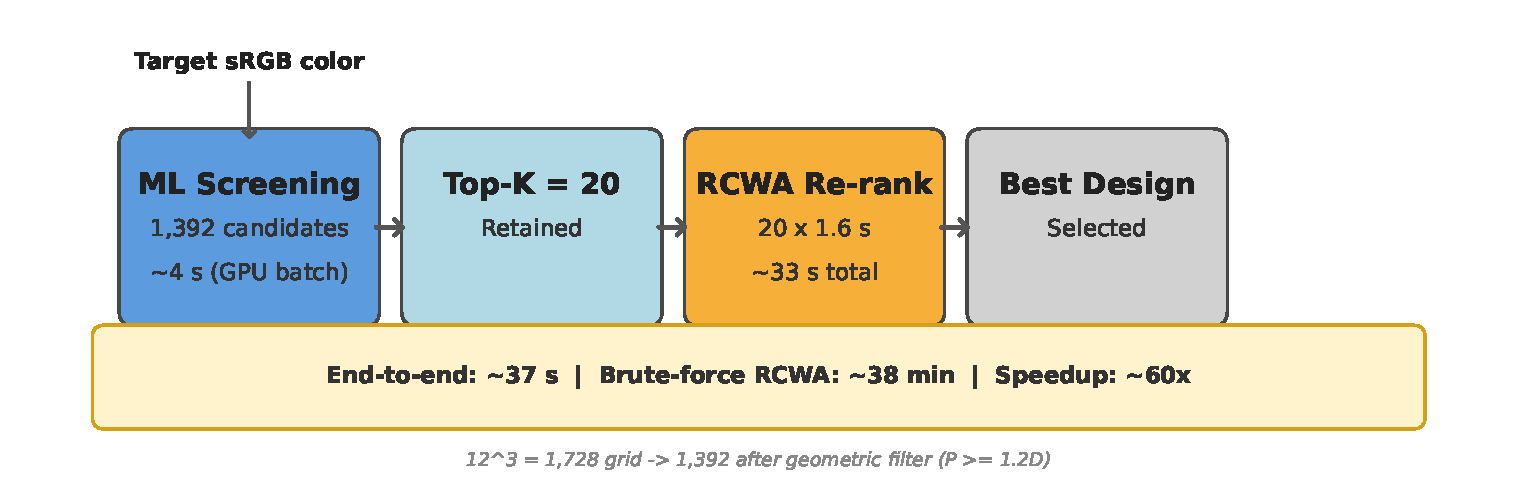
\includegraphics[width=0.9\figwidthDouble]{figures/fig1_protocol.pdf}
\caption{Closed-loop inverse design protocol. The ML surrogate screens 1392 candidates ($\sim$5~s GPU batch inference) and returns the top-$K = 20$; each undergoes independent RCWA verification ($\sim$33~s total); the verified best is selected.}
\label{fig:protocol}
\end{figure*}

The two-stage pipeline (Fig.~\ref{fig:protocol}) operates as follows. In Stage~1, a uniform $12^3 = 1728$-point grid over $(D, H, P)$ is screened by GPU batch inference ($\sim$5~s including color-difference computation); the top-$K = 20$ candidates by predicted CIEDE2000~\cite{ref16} are retained. In Stage~2, each candidate is re-evaluated by independent RCWA (nG = 65, Nxy = 256, $\sim$1.6~s each), and the RCWA-best is selected. Because the na\"ive ML pick is always contained in the top-$K$ pool, the hybrid satisfies $\Delta E_{\mathrm{hybrid}} \le \Delta E_{\mathrm{naive}}$ by construction.

End-to-end cost per target: $\sim$38~s (ML $\sim$5~s + RCWA $\sim$33~s), versus $\sim$38~min for brute-force 1392-call RCWA---a $\sim$60$\times$ speedup. All timings are measured on an Intel i7-14650HX / RTX 5060 Laptop workstation.

\subsection{Evaluation metrics}

Forward accuracy is measured as $\Delta E_{00}$ between ML-predicted and RCWA-computed colors on the frozen holdout set. Closed-loop achieved $\Delta E$ is computed as $\Delta E_{00}$(target, RCWA-verified result of the ML-selected design). The curse gap is defined as achieved $\Delta E - $ ML-claimed $\Delta E$. Thresholds: $\Delta E_{00} < 1.0$ (imperceptible); $< 2.3$ (just noticeable difference, JND).

\section{Results}

\subsection{Optimizer's curse and hybrid repair}

\begin{figure*}[!t]
\centering
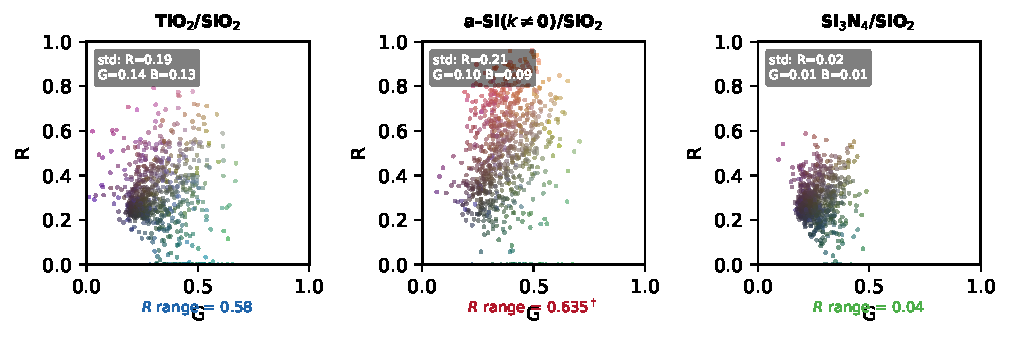
\includegraphics[width=\figwidthDouble]{figures/fig3_color_gamut.pdf}
\caption{sRGB color gamut of training sets. Left: TiO$_2$/SiO$_2$ (broad coverage). Center: a-Si/SiO$_2$ (absorption-confined). Right: Si$_3$N$_4$/SiO$_2$ (moderate gamut). Boxes give cross-sample sRGB standard deviations; subtitles give per-sample reflectance dynamic range ($R_{\max}-R_{\min}$, ensemble mean).}
\label{fig:gamut}
\end{figure*}

\subsubsection{TiO$_2$/SiO$_2$}

The TiO$_2$ ensemble achieves holdout $\Delta E_{00} = 2.99$ (mean; seed range 2.97--3.00), with 53\% of samples below the JND threshold (Table~\ref{tab:benchmark}).

An order-of-magnitude estimate from extreme value theory predicts the curse magnitude \textit{a priori}. If the surrogate's per-candidate prediction error has standard deviation $\sigma$ and the candidate pool size is $N$, the expected over-optimism of the rank-1 selection satisfies $\mathbb{E}[\mathrm{gap}] \approx \sigma\sqrt{2\ln N}$ (the expected maximum of $N$ independent Gaussian variables). For TiO$_2$ with $N = 1392$ (filtered grid), the amplification factor is $\sqrt{2\ln 1392} \approx 3.8$; with a per-candidate error std of $O(1)\ \Delta E_{00}$, the predicted over-optimism is $O(3$--$5)\ \Delta E_{00}$---the same magnitude as the measured median gap of $+3.59$ reported below. This order-of-magnitude consistency confirms that the curse is not an artifact of a particular model or dataset but a generic statistical consequence of optimizing over $O(10^3)$ noisy predictions.

Closed-loop tests use $N = 100$ roundtrip targets: geometries sampled from the same parameter distribution as the training data (uniform random sampling over $D,H,P$, with the same $D < P$ and fill-factor constraints), with their RCWA-simulated colors as inverse design targets. This protocol is non-circular: the targets are never used in surrogate training, the search grid ($12^3$ uniform, 1392 valid geometries) differs from the sampling distribution, the targets are colors rather than structure labels, and the final selection is validated by independent RCWA. The na\"ive ML strategy succeeds on only 19\% of targets, with a median curse gap of $+3.59\ \Delta E_{00}$. The ML systematically selects candidates whose prediction errors point in the favorable direction rather than genuinely optimal structures.

Hybrid re-ranking ($K = 20$) raises the success rate to 62\% (Wilson 95\% CI~\cite{ref18}: 52--71\%), with mean/median achieved $\Delta E$ of 2.18/1.83. The guarantee hybrid $\le$ na\"ive holds on all 100/100 targets. Paired McNemar tests confirm the hybrid gain is significant in all four main configurations (TiO$_2$/SiO$_2$, TiO$_2$/Al$_2$O$_3$, Si$_3$N$_4$, HfO$_2$; $p \le 2\times10^{-3}$, 400 targets, zero regressions). A controlled comparison on $N=100$ holdout targets---structures never seen by the surrogate---reproduces the success rate (63\%; Table~\ref{tab:a4}), ruling out memorization of training-set targets; the same ML screening beats a random-20 baseline by 63\% vs.\ 9\%, establishing that the surrogate's candidate ranking, not the RCWA re-verification alone, drives the gain. Convergence re-verification (nG $65 \to 101$) confirms 93\% of structures exhibit cross-order color change $<$ 1~JND (mean spread 0.64), excluding solver noise as an alternative explanation.

A complementary gamut-probing test ($N = 100$, targets sampled from the sRGB boundary) yields only 6\% hybrid success---most boundary colors lie outside TiO$_2$'s achievable gamut. The curse gap for these out-of-gamut targets is only $+0.81$ (median), versus $+3.59$ for in-gamut roundtrip targets, confirming that the curse amplifies only when candidates are closely spaced around reachable targets.

\subsubsection{a-Si/SiO$_2$ (complex index)}

The a-Si model achieves holdout $\Delta E_{00} = 2.37$ (seed-mean; seed range 2.31--2.45, $N = 1635$; the deployed 3-seed ensemble reaches 2.15), with 62\% below JND---the most accurate surrogate in this study. This accuracy is genuine: absorption-dominated spectral shapes are inherently easy to predict. The strongly absorbing index ($k \approx 0.77$ at 550~nm, up to 2.2 at 400~nm) compresses the achievable gamut: cross-sample sRGB std is only $R = 0.11$, $G = 0.08$, $B = 0.08$, and the per-sample reflectance dynamic range collapses to $R_{\max}-R_{\min} = 0.21$ (median) despite the material's high $\Delta n = 2.93$---absorption, not index contrast, caps the gamut.

Two closed-loop experiments probe the two sides of this narrow gamut. Gamut-probing targets ($N = 29$ fully-saturated hues, HSV $S = V = 0.95$, ${\approx}10^\circ$ hue spacing): 0\% success (binomial 95\% upper bound: 10\%; mean achieved $\Delta E = 22.4$), confirming that the sRGB boundary lies far outside the reachable gamut. Roundtrip targets ($N = 100$, in-gamut by construction): 86\% hybrid success at nG = 65, with mean/median achieved $\Delta E$ of 1.37/1.15 and a median curse gap of $+1.46$; a controlled holdout comparison reproduces 87\% vs.\ 4\% for a random-20 baseline (Table~\ref{tab:a4}).

The 86\%--not-0\% roundtrip rate within a severely restricted gamut demonstrates that roundtrip success measures in-gamut reachability, not gamut size: a-Si attains the highest measured success while probing the smallest gamut in this study, and its bare ML strategy already reaches 53\%. We caution that these success rates carry a solver-convergence caveat: cross-order re-verification (nG $65 \to 101$) confirms only 72\% of structures within 1~JND, and the success rate drops to 47\% at nG = 101 (nG = 131 probing still drifts; \S\ref{sec:convergence}). The high index contrast ($n = 4.39$) combined with strong absorption slows the RCWA Fourier convergence for this material specifically---lossless materials all confirm $\ge$93\% of structures---so a-Si design numbers must be read at fixed nG. This is, to our knowledge, the first systematic report of solver-order divergence for strongly absorbing high-index metasurface materials.

\begin{figure}[!t]
\centering
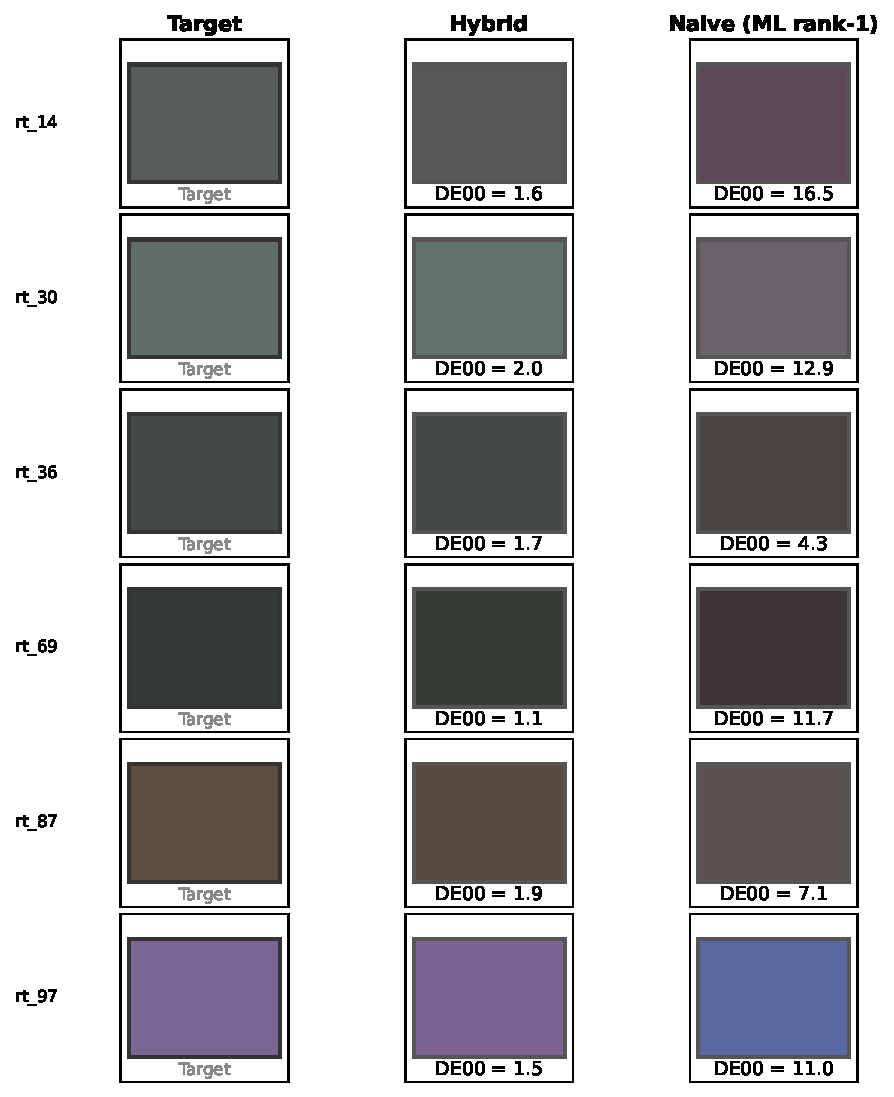
\includegraphics[width=0.85\figwidthSingle]{figures/fig_demo_colors.pdf}
\caption{Visual comparison of six roundtrip targets (TiO$_2$/SiO$_2$). Left: target color. Center: hybrid selection (RCWA-verified, $\Delta E_{00} = 1.1$--$2.0$). Right: na\"ive ML rank-1 selection ($\Delta E_{00} = 4.3$--$16.5$). The curse produces visible color shifts that hybrid re-ranking eliminates.}
\label{fig:demo}
\end{figure}

Fig.~\ref{fig:demo} provides a direct visual illustration: for six targets with large curse gaps, the hybrid selections are perceptually indistinguishable from the targets, while the na\"ive picks exhibit obvious color shifts---purple rendered as blue ($\Delta E_{00} = 11.0$), dark gray as purple-brown ($\Delta E_{00} = 16.5$).

\subsubsection{Summary}

\begin{table*}[!b]
\centering
\setlength{\tabcolsep}{3pt}
\caption{Inverse design benchmark. Success rates are hybrid (ML top-20 $+$ RCWA re-verification), JND threshold $\Delta E_{00} < 2.3$; $N=100$ roundtrip targets per configuration (probe: $N=29$). The nG101 re-verification column and the per-configuration convergence rate ($<$1~JND cross-order change) quantify solver-order robustness. Forward $\Delta E_{00}$ are seed-mean frozen-holdout values.}
\scriptsize
\label{tab:benchmark}
\begin{tabular}{@{}lccccccc@{}}
\toprule
Material & $\Delta n$ & Forward $\Delta E_{00}$ & RT @ nG65 & RT @ nG101 & Conv. & Probe & sRGB std \\
\midrule
a-Si/SiO$_2$ & 2.93 & 2.37$^{\dagger}$ & 86\%$^{\ddagger}$ & 47\%$^{\ddagger}$ & 72\% & 0\% & 0.11/0.08/0.08 \\
Si$_3$N$_4$/SiO$_2$ & 0.572 & 13.75$^{\S}$ & 81\% & 79\% & 98\% & --- & --- \\
TiO$_2$/SiO$_2$ & 0.958 & 2.99 & 62\%$^*$ & 53\% & 93\% & 6\% & --- \\
HfO$_2$/SiO$_2$ & 0.545 & 2.96 & 82\% & 80\% & 99\% & --- & --- \\
Ta$_2$O$_5$/SiO$_2$ & 0.652 & 3.04 & 74\% & 69\% & 95\% & --- & --- \\
GaN/SiO$_2$ & 0.938 & 2.89 & 66\% & 58\% & 94\% & --- & --- \\
Al$_2$O$_3$/SiO$_2$ & 0.313 & 8.11$^{\|}$ & 43\%$^{\S\S}$ & 43\% & 100\% & --- & --- \\
\midrule
TiO$_2$/Al$_2$O$_3$ & 0.645 & ---$^{\P}$ & 92\%$^{\S\S}$ & --- & --- & --- & --- \\
TiO$_2$/Si$_3$N$_4$ & 0.386 & ---$^{\P}$ & 96\%$^{\S\S}$ & --- & --- & --- & --- \\
\bottomrule
\end{tabular}

\vspace{2pt}
\raggedright\scriptsize $^*$Wilson 95\% CI: TiO$_2$ 52--71\%. $^{\dagger}$a-Si seed range 2.31--2.45 ($N=1635$); the deployed 3-seed ensemble reaches 2.15. $^{\ddagger}$nG = 65 verification; at nG = 101 the rate falls to 47\%, and nG = 131 probing still drifts (see \S\ref{sec:convergence})---a-Si rates must be read at fixed nG. $^{\S}$Si$_3$N$_4$ forward $\Delta E_{00}$ is independently reproduced on the frozen holdout ($N=5400$, aggregated over three substrates); the training-time validation-set estimate is deprecated. $^{\|}$Al$_2$O$_3$ single-seed surrogate. $^{\P}$TiO$_2$ substrate controls share the unified TiO$_2$ surrogate; substrate-specific forward holdout was not measured separately. $^{\S\S}$Wilson 95\% CI: Al$_2$O$_3$ 34--53\%, TiO$_2$/Al$_2$O$_3$ 85--96\%, TiO$_2$/Si$_3$N$_4$ 90--98\%. RT = roundtrip; probe = gamut-probe; Conv. = convergence rate (nG 65$\to$101, cross-order change $<$ 1~JND).
\end{table*}

\begin{table}[!t]
\centering
\setlength{\tabcolsep}{5pt}
\caption{Controlled comparison on holdout targets (structures never seen by the surrogate; $N = 100$ per arm, pre-registered JND threshold $\Delta E_{00} < 2.3$): naive (ML rank-1), hybrid (ML top-20 $+$ RCWA re-verification), and a random-20 baseline (20 uniformly sampled candidates $+$ RCWA re-verification).}
\footnotesize
\label{tab:a4}
\begin{tabular}{@{}lccc@{}}
\toprule
 & Naive & Hybrid & Random-20 \\
\midrule
TiO$_2$/SiO$_2$ & 24\% & 63\%$^{\dagger}$ & 9\% \\
a-Si/SiO$_2$ & 53\%$^{\ddagger}$ & 87\%$^{\S}$ & 4\% \\
\bottomrule
\end{tabular}

\vspace{2pt}
\raggedright\scriptsize $^{\dagger}$Wilson 95\% CI 53--72\%; vs.\ random-20 McNemar $b = 54, c = 0$, $p = 1.1\times10^{-16}$. $^{\ddagger}$$N = 96$ (4 naive RCWA failures). $^{\S}$Wilson 95\% CI 79--92\%; vs.\ random-20 McNemar $b = 83, c = 0$, $p = 2.1\times10^{-25}$. Roundtrip success on seen-structure targets matches holdout: TiO$_2$ 62\% vs.\ 63\%, a-Si 86\% vs.\ 87\% (Fisher $p = 1.0$), ruling out memorization.
\end{table}

\begin{figure*}[!t]
\centering
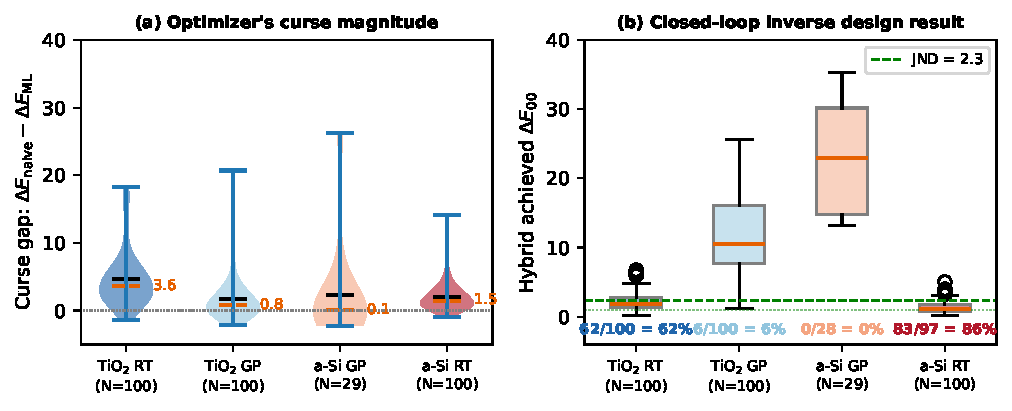
\includegraphics[width=\figwidthDouble]{figures/fig4_curse_gap.pdf}
\caption{Optimizer's curse and hybrid repair. (a) Curse-gap distributions; lines mark medians. (b) Hybrid achieved $\Delta E_{00}$ box plots. Dashed: JND threshold (2.3).}
\label{fig:curse}
\end{figure*}

Table~\ref{tab:benchmark} and Fig.~\ref{fig:curse} consolidate the test sets. The optimizer's curse is a $+2$--$+4\ \Delta E_{00}$ median over-optimism for in-gamut targets; hybrid re-ranking eliminates it deterministically; but re-ranking cannot expand the material's achievable gamut. Forward accuracy does not predict inverse design success: the least accurate surrogate (Si$_3$N$_4$, 13.75) attains 81\%, while the most accurate (a-Si, 2.37) reaches 86\%; a Spearman rank test across all seven dielectrics (seed-mean holdout forward accuracy, hybrid success rates) finds no significant association ($\rho = -0.43$, $p = 0.34$ at nG = 65; $\rho = +0.14$, $p = 0.76$ at nG = 101).

\subsection{Material screening criterion}

\begin{figure}[!t]
\centering
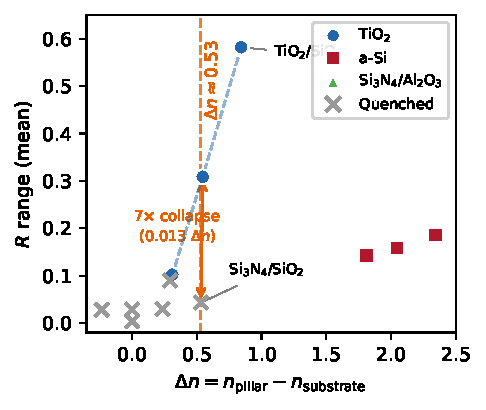
\includegraphics[width=\figwidthSingle]{figures/fig2_delta_n_criterion.pdf}
\caption{Material screening criterion, seven dielectrics on SiO$_2$. (a)~Reflectance dynamic range ($R_{\max}-R_{\min}$, per-sample, ensemble mean) vs.\ index contrast $\Delta n$ (550~nm): a resonance cutoff at $\Delta n \approx 0.5$ separates active materials ($R$ range $\ge 0.26$) from Al$_2$O$_3$, whose range collapses to 0.090. (b)~Hybrid roundtrip success vs.\ $\Delta n$ with Wilson 95\% CIs, including TiO$_2$ substrate controls (open symbols): roundtrip is anti-monotonic---TiO$_2$/Si$_3$N$_4$ ($\Delta n = 0.39$) reaches 96\% and Al$_2$O$_3$ reaches 43\% despite a degenerate gamut---so it is not a material screen.}
\label{fig:criterion}
\end{figure}

Across the seven primary datasets (each dielectric on SiO$_2$), reflectance dynamic range (per-sample $R_{\max} - R_{\min}$, ensemble mean) exhibits a sharp cutoff as a function of index contrast $\Delta n = n_{\mathrm{pillar}} - n_{\mathrm{substrate}}$. When $\Delta n$ drops below $\sim$0.5, the range collapses: HfO$_2$/SiO$_2$ and Si$_3$N$_4$/SiO$_2$ ($\Delta n = 0.545$ and 0.572) retain $R$ ranges of 0.264 and 0.290, while Al$_2$O$_3$/SiO$_2$ ($\Delta n = 0.313$) collapses to 0.090. Below threshold, guided modes degenerate into radiation modes and the structure reduces to a homogeneous thin film.

The same material on different substrates confirms the threshold: TiO$_2$ on SiO$_2$ / Al$_2$O$_3$ / Si$_3$N$_4$ gives $\Delta n = 0.958 / 0.645 / 0.386$ and $R$ range $= 0.582 / 0.309 / 0.102$, decreasing at an accelerating rate as $\Delta n$ approaches $\approx 0.5$.

Si$_3$N$_4$/SiO$_2$ ($\Delta n = 0.572$) confirms the criterion from above: with an $R$ range of 0.290 and an 81\% hybrid roundtrip success rate---comparable to HfO$_2$ (82\%)---it is an active, moderately saturated material rather than a zero-gamut limit. Al$_2$O$_3$/SiO$_2$ ($\Delta n = 0.313$) confirms the boundary from below through its resonance amplitude: the $R$ range collapses to 0.090, a factor of $\sim$3 below the weakest live material. Yet Al$_2$O$_3$ still attains 43\% hybrid roundtrip success ($N = 100$). This is not evidence of a useful gamut: roundtrip targets are sampled from the material's own parameter distribution, and a degenerate gamut is trivially self-consistent---because most geometries map to the same few dark, desaturated tones, a roundtrip target is reachable by many structures even though the surrogate is comparatively inaccurate overall (mean claimed $\Delta E \approx 7$). The roundtrip metric therefore measures in-gamut reachability, not gamut volume; the collapsed $R$ range, not the roundtrip rate, is what disqualifies Al$_2$O$_3$ as a structural-color material.

The substrate-variation controls make the point directly. Holding the pillar material fixed at TiO$_2$ and changing only the substrate traces $\Delta n = 0.958 / 0.645 / 0.386$ (SiO$_2$ / Al$_2$O$_3$ / Si$_3$N$_4$) against hybrid roundtrip success of 62\% / 92\% / 96\%: success \textit{rises} as $\Delta n$ \textit{falls}, and the lowest-contrast configuration ($\Delta n = 0.386$, below the resonance cutoff) attains the highest success of any system tested. The mechanism mirrors Al$_2$O$_3$: the lower-contrast configurations produce a simpler, more degenerate in-gamut color space, so their roundtrip targets are easy and the curse gap stays small (median $+0.75$ for TiO$_2$/Si$_3$N$_4$, versus $+3.59$ for TiO$_2$/SiO$_2$). Roundtrip success thus tracks in-gamut reachability and the surrogate's accuracy on those easy targets, not gamut size, and cannot serve as an \textit{a priori} material screen.

High $\Delta n$ alone does not guarantee a useful gamut. Despite the highest contrast (2.93), a-Si's color space is restricted by two loss mechanisms: impedance mismatch (excessive Fresnel reflection at the grating interface compresses resonant modulation) and material absorption ($k \approx 2.2$ at 400~nm removes blue-band photons; mean $R+T = 0.485$). The resulting sRGB std ($R = 0.11$, $G = 0.08$, $B = 0.08$) supports only dark reds and browns.

Synthesizing all datasets, we propose a two-stage screening criterion (Fig.~\ref{fig:criterion}): (i)~necessary condition: $\Delta n \gtrsim 0.5$ for resonance existence---the reflectance dynamic range collapses below this threshold (Al$_2$O$_3$, $R$ range 0.090), whereas every lossless dielectric with $\Delta n \ge 0.54$ retains $R$ range $\ge 0.26$ and supports an active gamut; (ii)~sufficient condition: low extinction ($k \approx 0$) combined with moderate index ($n \approx 2.0$--2.5) for maximum gamut. TiO$_2$ satisfies both; a-Si satisfies (i) but fails (ii); Al$_2$O$_3$ fails (i)---its 43\% roundtrip success notwithstanding, because that metric reflects in-gamut reachability rather than gamut volume.

\section{Discussion}

\subsection{Mechanism: why hybrid repairs the curse, and when the pool is empty}

The three-stage causal chain explains both the curse and its repair. First, for the lossless materials the 1392 grid candidates contain none close to a typical roundtrip target (all lie at $\Delta E_{00} \sim 10$--$15$), and the separations between neighboring candidates within this cluster are comparable to the ML error ($\sim$3 for TiO$_2$). The ranking of the leading candidates is therefore noise-dominated---the surrogate cannot distinguish genuinely better structures from ones whose prediction error happens to be favorable---so the na\"ive rank-1 pick is effectively random. Second, hybrid re-ranking of the top-20 is equivalent to drawing 20 candidates and selecting the best-verified. For TiO$_2$, the 62\% success rate implies $\sim$5\% of grid candidates ($\sim$67 per target) lie within JND---the pool contains answers, and RCWA verification finds them. The controlled random-20 baseline (Table~\ref{tab:a4}) confirms that this is not an artifact of pool density alone: 20 random candidates succeed on only 9\% (TiO$_2$) and 4\% (a-Si) of targets, so the surrogate's ranking, not the verification step, is what concentrates the pool's sparse viable candidates into the top-20. Third, when the pool genuinely contains no viable candidate---a-Si gamut-probing targets, which lie far outside the absorbing material's narrow gamut---even perfect re-ranking cannot succeed (0\%).

The optimizer's curse is curable; the material limit is not. Better verification raises success toward the pool ceiling; better material selection raises the ceiling itself.

Among lossless materials, the highest success rates occur at moderate index contrast: HfO$_2$ ($\Delta n = 0.545$) and Si$_3$N$_4$ ($\Delta n = 0.572$) reach 82\% and 81\%, exceeding TiO$_2$ (62\%) and GaN (66\%) at $\Delta n \approx 0.94$--0.96. Weaker resonances yield smoother, simpler spectral responses that the surrogate predicts more accurately, so forward accuracy translates more directly into design success; high-$\Delta n$ systems support sharper resonances whose prediction is more error-prone, partially offsetting their larger gamut. The absorbing a-Si (86\% at nG = 65) breaks this pattern only within its dark, low-saturation gamut, where absorption-dominated spectra are easy to predict and the in-gamut candidate pool is dense.

\subsection{Solver convergence}
\label{sec:convergence}

\begin{figure*}[!t]
\centering
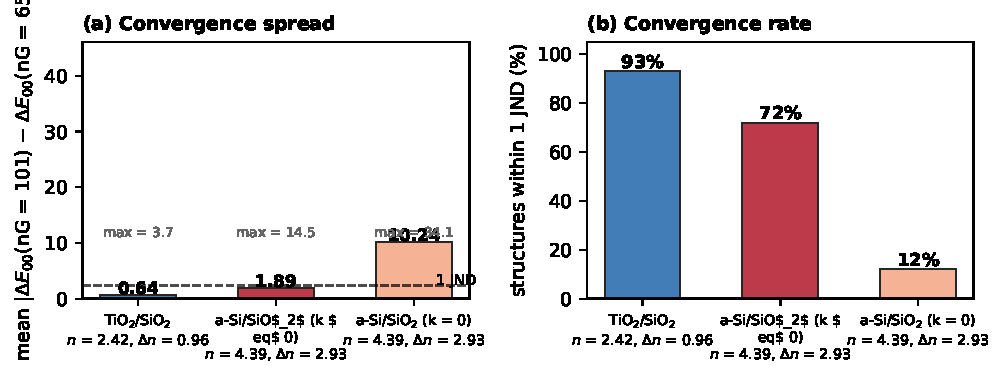
\includegraphics[width=\figwidthDouble]{figures/fig5_nG_convergence.pdf}
\caption{RCWA convergence (nG $65 \to 101$). (a) Mean per-structure color spread. (b) Fraction within 1~JND. Lossless dielectrics converge ($\ge$93\% within 1~JND); the strongly absorbing a-Si does not (72\%, spread 1.89), and removing its absorption (k = 0) degrades convergence further to 12\% (spread 10.24).}
\label{fig:convergence}
\end{figure*}

The nG convergence test (Fig.~\ref{fig:convergence}) reveals strong material dependence: lossless materials confirm $\ge$93\% of structures within 1~JND across nG $65 \to 101$ (TiO$_2$ 93\%, mean spread 0.64; Si$_3$N$_4$ 98\%; HfO$_2$ 99\%; Ta$_2$O$_5$ 95\%; GaN 94\%; Al$_2$O$_3$ 100\%), whereas the strongly absorbing a-Si confirms only 72\% (mean spread 1.89, max 14.47) and its success rate falls from 86\% (nG 65) to 47\% (nG 101). A $k = 0$ control---the same index profile with extinction removed---degrades convergence further to 12\% (spread 10.24, max 34.09): absorption damps the sharp, high-$Q$ resonances that Fourier truncation corrupts, so the lossy system converges better than its lossless counterpart. The remaining a-Si deficit relative to lossless moderate-index materials is driven by the high index contrast ($n = 4.39$), whose sharp permittivity discontinuities decay slowly in Fourier space. For lossless moderate-index materials ($n \approx 2.0$--$2.5$), nG = 65 suffices; for strongly absorbing high-index systems, success rates must be reported at fixed nG---a caveat we make explicit in Table~\ref{tab:benchmark}.

\subsection{Capability boundaries}

Hybrid re-ranking eliminates statistical bias but not systematic error: the surrogate's baseline accuracy (TiO$_2$ $\sim$3, a-Si $\sim$2.4 $\Delta E_{00}$, seed-mean) is determined by architecture, data quality, and material physics, and cannot be improved by re-ranking. The method is bounded by pool coverage---if the global optimum lies outside the searched grid, re-ranking returns only the pool-best.

\textbf{Robustness of the cutoff to the index metric.} The threshold $\Delta n \approx 0.5$ is insensitive to the convention used to quantify the index contrast. Throughout this work $\Delta n$ is defined relative to the film index at the central visible wavelength, $\Delta n = n(550\,\mathrm{nm}) - n_{\mathrm{sub}}$; an equally common convention uses the Cauchy asymptote $A$ (the $\lambda\to\infty$ limit) as the film index. Because all six dielectrics exhibit normal dispersion ($B>0$), $n(550\,\mathrm{nm})$ exceeds $A$ by 0.02--0.13, so the two metrics order the materials identically and shift every point by only a small, monotonic offset. Critically, the classification boundary is unaffected: the dead material Al$_2$O$_3$ and the weakest live material HfO$_2$ are separated by $\Delta n = 0.30 \to 0.51$ under the Cauchy-$A$ convention and by $0.31 \to 0.54$ under the $n(550\,\mathrm{nm})$ convention. In both conventions the cutoff at $\Delta n \approx 0.5$ falls inside the gap between the dead and live materials, so the dead/live assignment---and the resulting two-stage screening rule---does not depend on which reference wavelength is chosen. We adopt $n(550\,\mathrm{nm})$ because it references the wavelength at which the inverse-design color error is evaluated, but this choice is one of convenience rather than necessity.

Sensitivity to $K$: for TiO$_2$ roundtrip, success rises from 47\% ($K = 5$) through 57\% ($K = 10$) to 62\% ($K = 20$), then saturates at 64\% ($K = 50$)---a 2-percentage-point gain at 2.5$\times$ cost; HfO$_2$ exhibits the same knee (68\%, 75\%, 82\% at $K = 5$, 10, 20). $K = 20$ sits at the knee of the cost--accuracy curve.

Our work targets the ML-surrogate-plus-verification paradigm. Alternative approaches---topology optimization and adjoint methods~\cite{ref25,ref26}, generative models~\cite{ref27}---avoid surrogate bias by iterating with full-wave solvers or learning the inverse mapping directly, but at higher computational or data cost. The core insight here---that optimization over a noisy objective amplifies error---is not specific to photonics and would manifest in any paradigm where an approximate model guides selection.

\subsection{Practical guidelines}

Four rules follow from these results. (1)~Before training, compute $\Delta n$; if $< 0.5$, the material cannot support guided-mode resonances of useful amplitude ($R$ range collapses below $\sim$0.1) and yields no practical structural-color gamut---irrespective of how high its roundtrip success appears, since that metric only reflects recovery of the material's own degenerate colors. (2)~Never judge inverse design capability from forward $\Delta E$ alone; always perform closed-loop verification. (3)~Adopt hybrid re-ranking with $K \ge 20$; the $\sim$38~s cost eliminates the $+2$--$4\ \Delta E_{00}$ over-optimism at negligible overhead versus brute force. (4)~If roundtrip success falls below $\sim$30\%, the bottleneck is pool density---expand the geometry space or switch materials rather than tuning the network.

\subsection{Limitations}

The present study is limited to cylindrical nanopillars under normal-incidence TE polarization; elliptical, multilayer, or wide-angle geometries may expand the gamut. All results are numerical (RCWA); fabrication imperfections (sidewall taper, roughness) may introduce additional error. a-Si optical constants vary with deposition conditions; deployment should use process-matched measurements. Angular-resolved and multi-polarization inverse design validation remain future work.

\section{Conclusion}

We have established a closed-loop validation framework for ML-assisted metasurface structural color inverse design. Three results emerge: (1)~forward prediction accuracy is necessary but insufficient for inverse design success---candidate pool density is the sufficient condition; (2)~the optimizer's curse produces a $+2$--$4\ \Delta E_{00}$ median over-optimism for in-gamut targets that hybrid re-ranking eliminates deterministically (hybrid $\le$ na\"ive on all targets across seven dielectrics); (3)~a resonance cutoff at $\Delta n \approx 0.5$ provides an \textit{a priori} material screening criterion---the reflectance dynamic range collapses below it (Al$_2$O$_3$, $R$ range 0.090), whereas five lossless dielectrics spanning $\Delta n = 0.54$--0.96 retain $R$ range $\ge 0.26$ and achieve 62--82\% hybrid roundtrip success (365/500 = 73\% combined). Crucially, the screen rests on resonance amplitude, not on roundtrip success: Al$_2$O$_3$ still reaches 43\% roundtrip and TiO$_2$/Si$_3$N$_4$ ($\Delta n = 0.39$) reaches 96\%, confirming that roundtrip measures in-gamut reachability rather than gamut volume; absorbing a-Si remains severely gamut-limited.

The framework yields a testable prediction: for any lossless dielectric with $\Delta n > 0.6$, hybrid roundtrip success should exceed 50\% at $K = 20$, provided the grid covers $\ge$1000 valid structures. More broadly, the extreme-value estimate $\sigma\sqrt{2\ln N}$ and the closed-loop protocol apply to surrogate-assisted optimization beyond photonics---any workflow selecting the best candidate from a noisy predictor benefits from the same diagnosis and repair.

\section*{Funding}
[To be inserted by corresponding author.]

\section*{Disclosures}
The authors declare no conflicts of interest.

\section*{Author contributions}
A.Q. conceived the study, developed the methodology, performed all simulations and data analysis, and wrote the manuscript. [Advisor contributions to be added.]

\section*{Data availability}
Data underlying the results presented in this paper are not publicly available at this time but may be obtained from the corresponding author upon reasonable request.

\begin{thebibliography}{99}
\bibitem{ref1} S. Kinoshita, S. Yoshioka, and J. Miyazaki, ``Physics of structural colors,'' Rep. Prog. Phys. \textbf{71}, 076401 (2008).
\bibitem{ref4} A. I. Kuznetsov, A. E. Miroshnichenko, M. L. Brongersma, Y. S. Kivshar, and B. Luk'yanchuk, ``Optically resonant dielectric nanostructures,'' Science \textbf{354}, aag2472 (2016).
\bibitem{ref6} M. G. Moharam and T. K. Gaylord, ``Rigorous coupled-wave analysis of planar-grating diffraction,'' J. Opt. Soc. Am. \textbf{71}, 811--818 (1981).
\bibitem{ref7} A. Taflove and S. C. Hagness, \textit{Computational Electrodynamics}, 3rd ed. (Artech House, 2005).
\bibitem{ref8} S. Molesky, Z. Lin, A. Y. Piggott, W. Jin, J. Vuckovi\'c, and A. W. Rodriguez, ``Inverse design in nanophotonics,'' Nat. Photonics \textbf{12}, 659--670 (2018).
\bibitem{ref12} D. T. Pierce and W. E. Spicer, ``Electronic structure of amorphous Si from photoemission and optical studies,'' Phys. Rev. B \textbf{5}, 3017--3025 (1972).
\bibitem{ref13} D. R. Jones, M. Schonlau, and W. J. Welch, ``Efficient global optimization of expensive black-box functions,'' J. Global Optim. \textbf{13}, 455--492 (1998).
\bibitem{ref14} J. Gonzalez, Z. Dai, P. Hennig, and N. Lawrence, ``Batch Bayesian optimization via local penalization,'' in \textit{Proc. AISTATS} (2016).
\bibitem{ref15} R. Magnusson and S. S. Wang, ``New principle for optical filters,'' Appl. Phys. Lett. \textbf{61}, 1022--1024 (1992).
\bibitem{ref16} G. Sharma, W. Wu, and E. N. Dalal, ``The CIEDE2000 color-difference formula: implementation notes, supplementary test data, and mathematical observations,'' Color Res. Appl. \textbf{30}, 21--30 (2005).
\bibitem{ref17} W. Fan and grcwa contributors, ``grcwa: Python library for rigorous coupled-wave analysis,'' \url{https://github.com/fancompute/grcwa} (2023).
\bibitem{ref18} E. B. Wilson, ``Probable inference, the law of succession, and statistical inference,'' J. Am. Stat. Assoc. \textbf{22}, 209--212 (1927).
\bibitem{ref19} G. Shao, T. Zhou, T. Yan, Y. Guo, Y. Zhao, R. Huang, and L. Fang, ``Reliable, efficient, and scalable photonic inverse design empowered by physics-inspired deep learning,'' Nanophotonics \textbf{14}, 20240456 (2025).
\bibitem{ref20} R. Marzban, A. Adibi, and R. Pestourie, ``Inverse design in nanophotonics via representation learning,'' Adv. Opt. Mater. \textbf{14}, 2501871 (2026).
\bibitem{ref21} H. Lee, H. Moon, J. Lee, and S. Ryu, ``Toward knowledge-guided AI for inverse design in manufacturing,'' Adv. Intell. Discov. \textbf{2}, 2500107 (2025).
\bibitem{ref22} D. Russo, ``Simple Bayesian algorithms for best-arm identification,'' Oper. Res. \textbf{68}, 1625--1647 (2020).
\bibitem{ref23} D. Liu, Y. Tan, E. Khoram, and Z. Yu, ``Training deep neural networks for the inverse design of nanophotonic structures,'' ACS Photonics \textbf{5}, 1365--1369 (2018).
\bibitem{ref24} I. Malkiel, M. Mrejen, A. Nagler, U. Arieli, L. Wolf, and H. Suchowski, ``Plasmonic nanostructure design and characterization via deep learning,'' Light: Sci. Appl. \textbf{7}, 60 (2018).
\bibitem{ref25} A. Y. Piggott, J. Lu, K. G. Lagoudakis, J. Petykiewicz, T. M. Babinec, and J. Vu\v{c}kovi\'c, ``Inverse design and demonstration of a compact and broadband on-chip wavelength demultiplexer,'' Nat. Photonics \textbf{9}, 374--377 (2015).
\bibitem{ref26} R. E. Christiansen and O. Sigmund, ``Inverse design in photonics by topology optimization: tutorial,'' J. Opt. Soc. Am. B \textbf{38}, 496--509 (2021).
\bibitem{ref27} Z. Ma, S. M. Hanham, P. Albella, B. Ng, H. T. Tan, M. Hong, and Y. F. Lu, ``Deep learning enabled inverse design in nanophotonics,'' Nanophotonics \textbf{9}, 1041--1057 (2020).
\bibitem{ref28} B. Cai, X. Huang, H. Zhang, J. Sun, and T. J. Cui, ``Deep learning and structural color,'' Appl. Phys. Lett. \textbf{119}, 020501 (2021).
\bibitem{ref29} A. S. Barker and M. Ilegems, ``Infrared lattice vibrations and free-electron dispersion in GaN,'' Phys. Rev. B \textbf{7}, 743--750 (1973).
\bibitem{ref30} E. D. Palik, \textit{Handbook of Optical Constants of Solids} (Academic Press, San Diego, 1998).
\bibitem{ref31} J. M. Khoshman, A. Khan, and M. E. Kordesch, ``Amorphous hafnium oxide thin films for antireflection optical coatings,'' Surf. Coat. Technol. \textbf{202}, 2500--2502 (2008).
\end{thebibliography}

\end{document}
